\documentclass{article}

\usepackage{../preamble}
\standalonetrue

\pagestyle{fancy}
\fancyhf{}
\rhead{Section \thesection}
\lhead{PHYS 304 Lecture 21}
\rfoot{Page \thepage}


\title{PHYS 304 Lecture 21}
\author{Ashtan Mistal}
\date{!!!}

\begin{document}

\ifstandalone
\maketitle
\fi

\graphicspath{{./Lecture21/}}

\section{Key review of points from last lecture}

We derived the radial and angular contributions to the orthonormal eigen states of the hydrogen atom Hamiltonian, and found that the requirement for a bounded solution in r put constraints on the energy eigenvalues such that $E_n = \frac{E_1}{n^2}$, where $E_1$ is negative. 

The full eigen functions, $\psi_{nlm}(r, \theta, \phi) = R_{nl}(r) Y_l^m(\theta,\phi)$, where

% finish from slides

\section{Today: Zoology of full eigen function quantum numbers for the hydrogen atom Hamiltonian}


\begin{itemize}
    \item Keep track of the nodes!
\end{itemize}
    $$\psi_{nlm}(r, \theta, \phi) = R_{nl}(r) Y_l^m(\theta,\phi)$$
    
    $$R_{nl}(r) = \frac{1}{r} \rho^{l+1} e^{-\rho} \nu(\rho), \quad \nu(\rho) = \sum_{j=0}^\infty a_j \rho^j$$
    
    Recall that the spherical harmonics have a total of $l$ nodes in the angular degrees of freedom.
    
    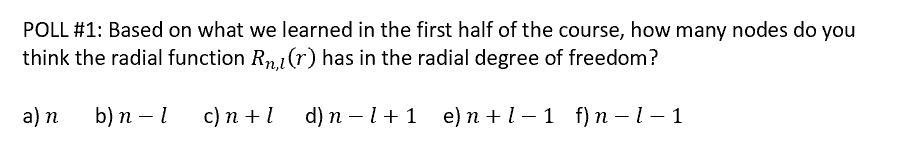
\includegraphics[width = 0.8 \textwidth]{Lecture21/1.png}
    
    Based on first half of course, each distinct energy eigen state has a distinct number of nodes $(n-1)$.  Thus since $Y_l^m$ has $l$ nodes, expect $R_n^l$ to have $n-1-l$ nodes.
    
    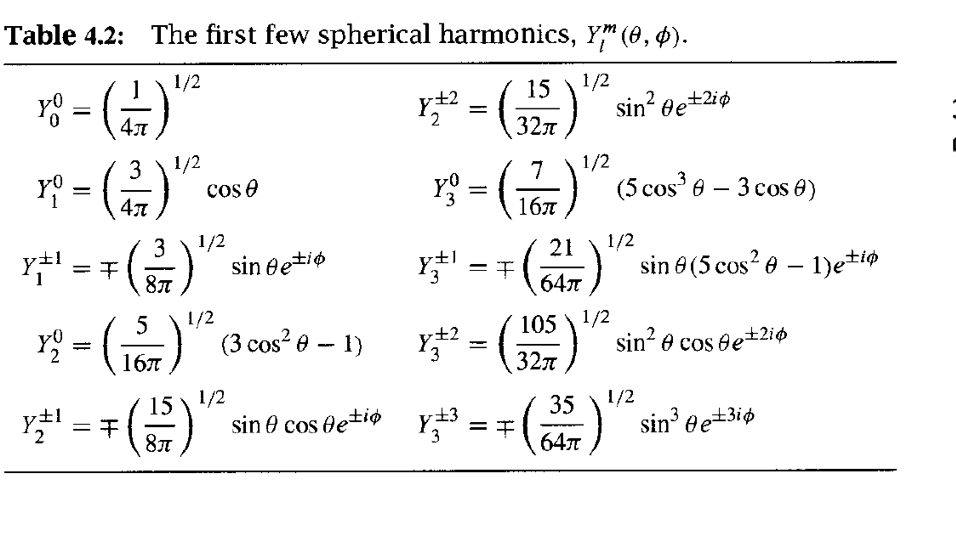
\includegraphics[width = 0.7 \textwidth]{Lecture21/2.png}
    
    
    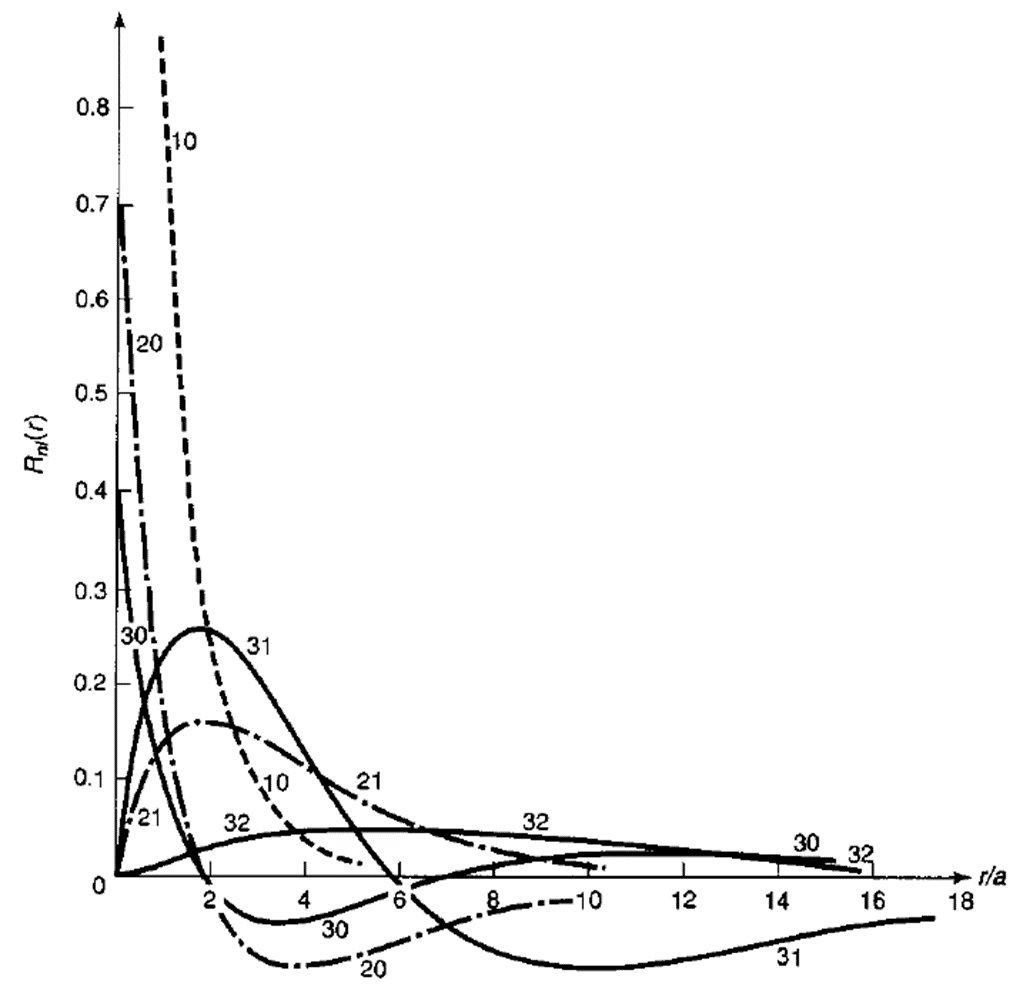
\includegraphics[width = 0.7 \textwidth]{Lecture21/3.png}
    
    Degeneracy of an energy eigen state associated with a given n value?

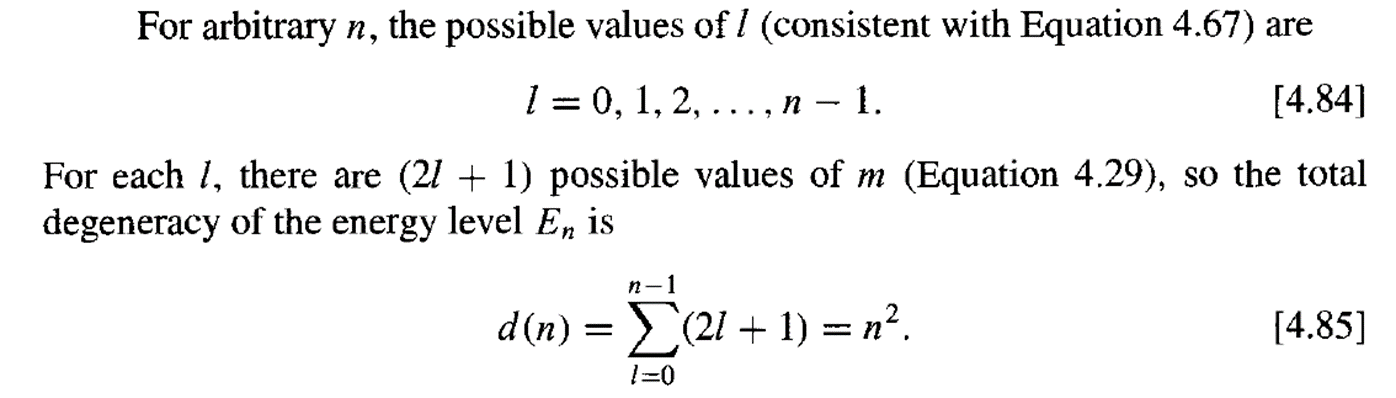
\includegraphics[width = 0.7 \textwidth]{Lecture21/4.png}

Equation 4.67: $R_{nl}$ bounded

Equation 4.29: $P_l^m(\cos(\theta))$

Only the n quantum number determines the energy of the n2 in number states with consistent values of integer $\ell$, $0 \leq \ell \leq n$, and for each $\ell$, $m=-\ell, -\ell+1,...0,...,\ell$ ($2\ell+1$ in number). 

\subsection*{Useful table:}

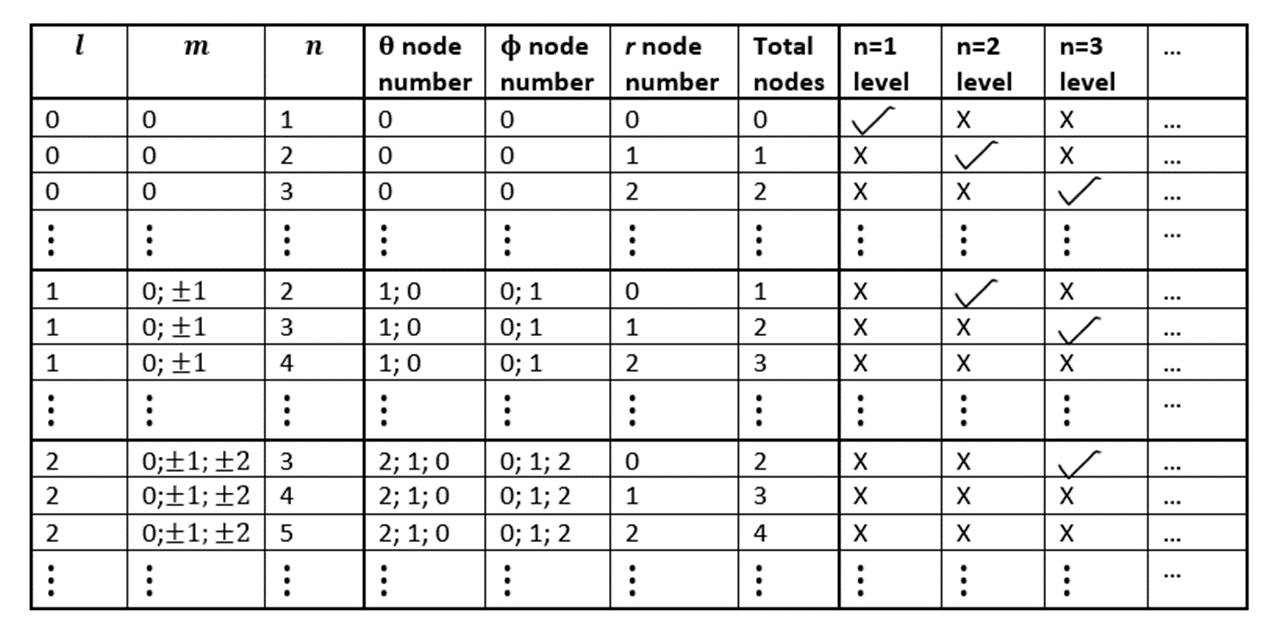
\includegraphics[width = 0.94 \textwidth]{Lecture21/5.png}

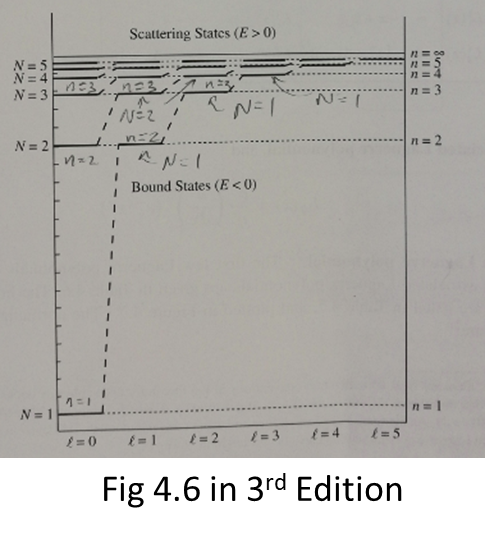
\includegraphics[width = 0.7 \textwidth]{Lecture21/6.png}

If you could see visible light being emitted from a florescent tube filled only with hydrogen, what can you say about the stationary states that are likely somehow involved in the corresponding light emission process within the hydrogen atoms?

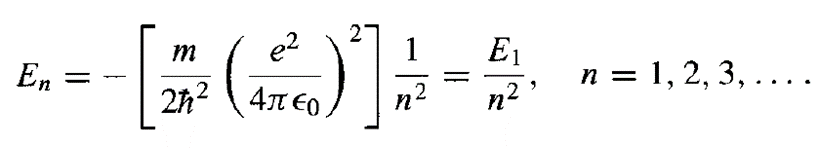
\includegraphics[width = 0.6 \textwidth]{Lecture21/7.png}

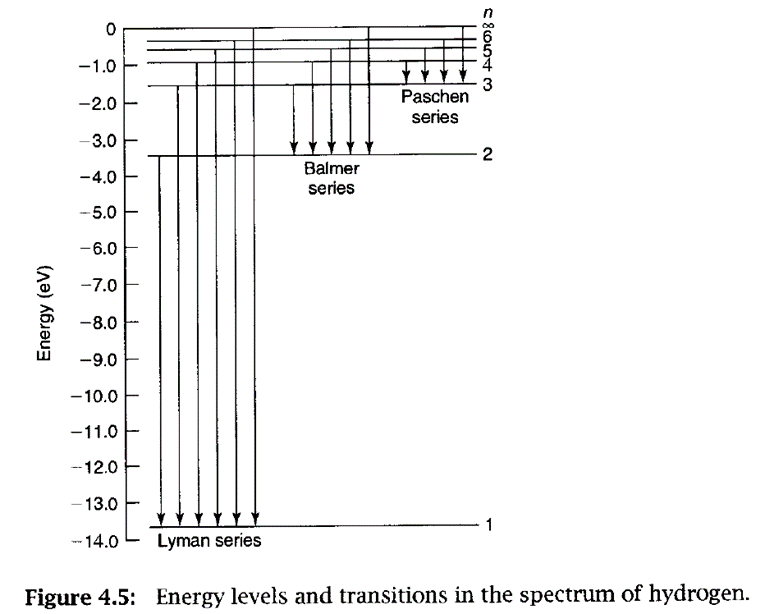
\includegraphics[width = 0.94 \textwidth]{Lecture21/8.png}

\section{Angular Momentum Operators}

At this point in the course, if I asked “what type of wavefunction represents a particle with linear momentum?”, what would you answer?



In classical mechanics, what is the angular momentum equivalent to the linear momentum expression for a particle $p = m \frac{dx}{dt}$



Combining these answers, which parts of our hydrogen atom eigen functions seem to be directly related to angular momentum?



Which component of angular momentum?

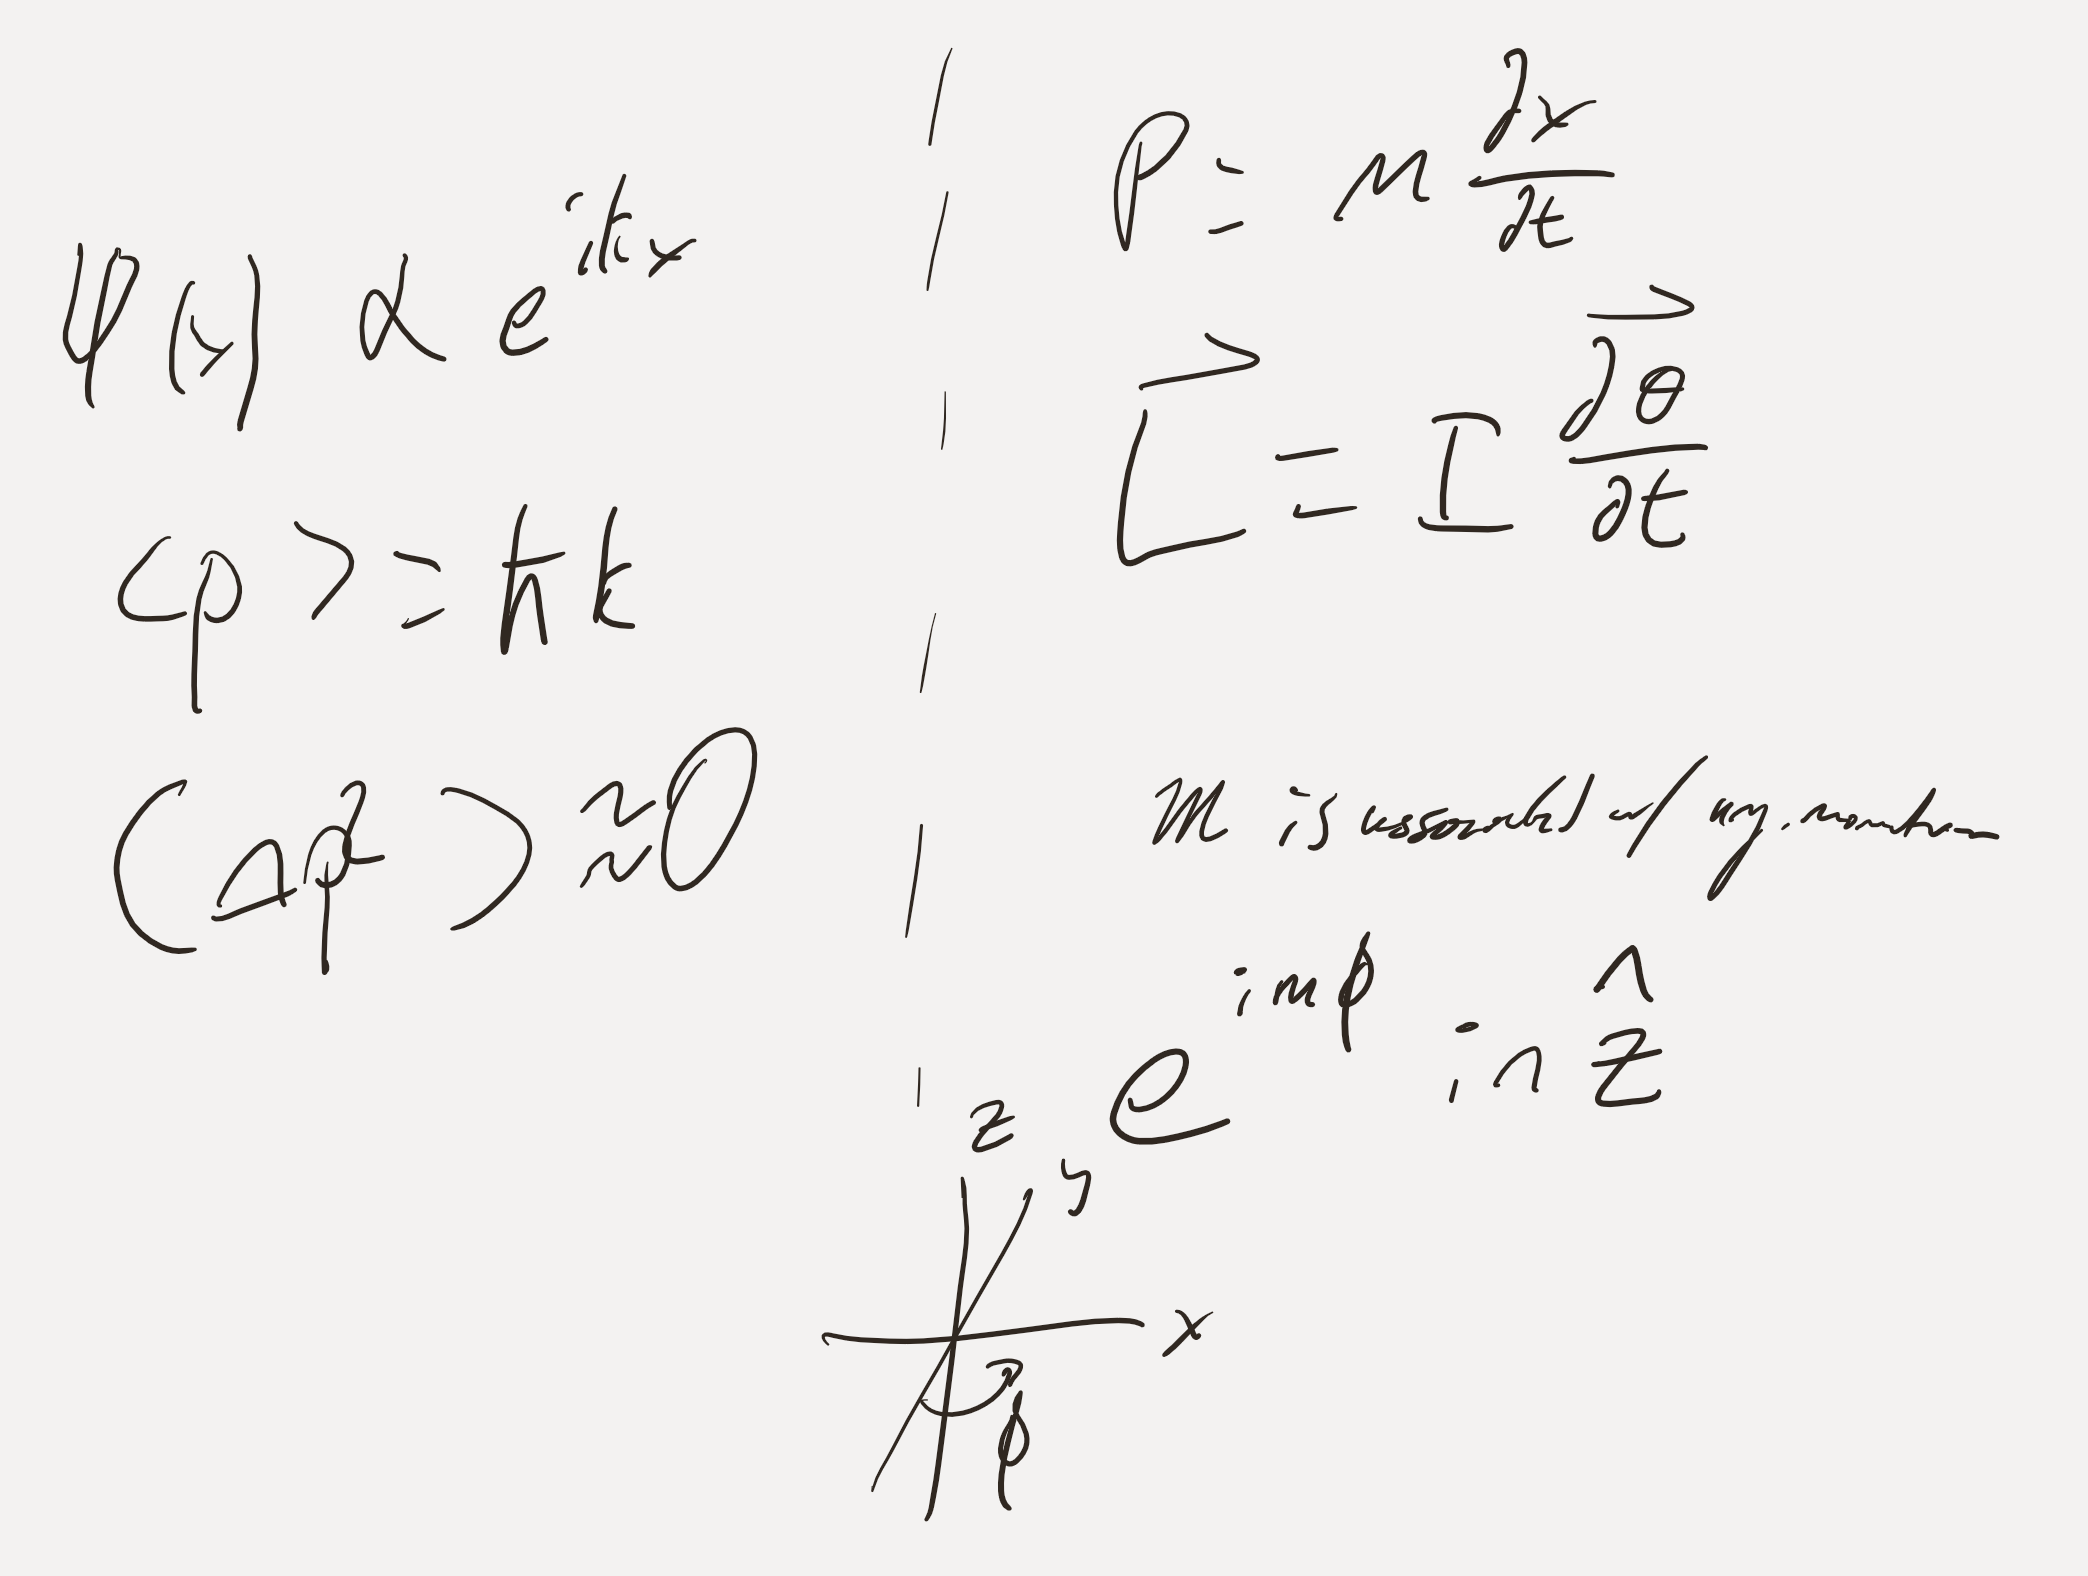
\includegraphics[width = 0.95 \textwidth]{Lecture21/9.png}

The angular momentum operator in the position basis, using cartesian coordinates:

$$\hat{\vec{L}} = \hat{\vec{r}} \times \hat{\vec{p}}$$

In the position basis:

$$\hat{\vec{L}}  = \vec{r} \times \hat{\vec{p}}$$

$$\left| \begin{matrix} i & j & k \\ x & y & z \\ p_x & p_y & p_z \end{matrix} \right|$$

Cartesian coordinates:

$$\hat{\vec{L}} = -i \hbar \left\{ \left( y \frac{d}{dz} - z \frac{d}{dy} \right) \hat{i} - \left( x \frac{d}{dz} - z \frac{d}{dx} \right) \hat{j} - \left( x \frac{d}{dy} - y \frac{d}{dx} \right) \hat{k} \right\}$$

$$[\hat{L}_x, \hat{L}_y] = \hbar^2 \left[ \left( y \frac{d}{dz} - z \frac{d}{dy} \right), \left( x \frac{d}{dz} - z \frac{d}{dx} \right) \right]$$

$$ = \hbar^2 \left\{ 
\underbrace{\left[ y \frac{d}{dz}, x \frac{d}{dz} \right]}_{=0} - 
\left[ y \frac{d}{dz}, z \frac{d}{dx} \right] - 
\left[ z \frac{d}{dy}, x \frac{d}{dz} \right] + 
\underbrace{\left[ z \frac{d}{dy}, x \frac{d}{dx} \right]}_{=0} \right\}$$

$$ = \hbar^2 \left( -y \frac{d}{dx} + x \frac{d}{dy} \right)$$

$$ = i \hbar \hat{L}^2$$

Cyclic permutation $\Rightarrow$  $[\hat{L}_y, \hat{L}_z] = i \hbar \hat{L}_x$, $[\hat{L}_z, \hat{L}_x] = i \hbar \hat{L}_y$

Define $$|\hat{\vec{L}}^2 = \hat{L}^2 = \hat{L}_x + \hat{L}_y + \hat{L}_y$$

$$\Rightarrow [\hat{L}^2, \hat{L}_x] = [\hat{L}_y^2, \hat{L}_x] + [\hat{L}_z^2, \hat{L}_x]  = \hat{L}_y [ \hat{L}_y,\hat{L}_x] + [ \hat{L}_y,\hat{L}_x] \hat{L}_y + 
\hat{L}_z [ \hat{L}_z,\hat{L}_x] + [ \hat{L}_z,\hat{L}_x] \hat{L}_z  = 0$$

(change into corresponding $i \hbar \hat{L}_{...}$)

$$\Rightarrow [\hat{L}^2, \hat{L}_i] = 0, \quad i = x,y,x$$

$\hat{L}^2$ commutes with any of $\hat{l}_x, \hat{L}_y,$ or $\hat{L}_z$ so $\hat{L}^2$ can share eigen states / functions with one of $\hat{l}_x, \hat{L}_y,\hat{L}_z$ (measure $\hat{L}^2 + \hat{L}_z \Rightarrow$ in a common eigen state of $\hat{L}^2 + \hat{L}_z$ BUT since $[\hat{L}_z, \hat{L}_x (or) \hat{L}_y] \neq 0$

$\Rightarrow$ that common eigen state of $\hat{L}^2 + \hat{L}_z$ will have some nonzero variance in $\hat{L}_x, \hat{L}_y \Rightarrow$ can't "know" $\braket{\hat{\vec{L}}}$ precisely. \textbf{IMPORTANT!!}

Now ask: 

$$\hat{L}_\pm = \hat{L}_x \pm i \hat{L}_y$$

The angular momentum ladder operators: how do they commute?

$$[\hat{L}^2, \hat{L}_\pm] = 0$$

$$[\hat{L}^2, \hat{L}_\pm] = [\hat{L}_z, \hat{L}_x] \pm i  [\hat{L}_z, \hat{L}_y]$$

$$= i\hbar \hat{L}_y \pm i (- i \hbar L_x)$$

$$= \pm \hbar \hat{L}_\pm$$





\end{document}